% answers.tex —— 2006 年·普通高等学校招生考试·江苏卷 · 参考答案与详细解析片段
% 由 tools/generate_projects.py 依来源总账自 2006/2006_数学真题_江苏_试题.md + 2006/2006_数学真题_江苏_解析正文.md + 2006/2006_数学真题_江苏_答案要点.md 生成，勿手改（改源 MD 后重跑）


\begin{gktip}
下列推导只依据固定候选题面及题图，是本库独立非官方草稿，已由第二人按固定 PDF 完成全卷盲核。未引用或补入外部答案；逐题 provenance 尚待录入，不代表官方答案或评分标准。
\end{gktip}

\begin{answer}
\gksolhead{1}{}

\textbf{题目}：

已知 $a\in\mathbb R$，函数 $f(x)=\sin x-|a|$，$x\in\mathbb R$ 为奇函数，则 $a=$\mbox{（　　）}

\begin{gkopts}(4)
\task （A）$0$
\task （B）$1$
\task （C）$-1$
\task （D）$\pm1$
\end{gkopts}

\Needspace{4\baselineskip}
\textbf{解析}

若 $f$ 为奇函数，则 $f(0)=0$。而 $f(0)=-|a|$，故 $a=0$。

\gkanswer{答案：A（$a=0$）。}

\end{answer}
\begin{answer}
\gksolhead{2}{}

\textbf{题目}：

圆 $(x-1)^2+(y+\sqrt3)^2=1$ 的切线方程中有一个是\mbox{（　　）}

\begin{gkopts}(4)
\task （A）$x-y=0$
\task （B）$x+y=0$
\task （C）$x=0$
\task （D）$y=0$
\end{gkopts}

\Needspace{4\baselineskip}
\textbf{解析}

圆心为 $(1,-\sqrt3)$、半径为 $1$。选项 $x=0$ 到圆心的距离为 $1$，故该直线为切线。

\gkanswer{答案：C。}

\end{answer}
\begin{answer}
\gksolhead{3}{}

\textbf{题目}：

某人 5 次上班途中所花的时间（单位：分钟）分别为 $x,y,10,11,9$。已知这组数据的平均数为 $10$，方差为 $2$，则 $|x-y|$ 的值为\mbox{（　　）}

\begin{gkopts}(4)
\task （A）$1$
\task （B）$2$
\task （C）$3$
\task （D）$4$
\end{gkopts}

\Needspace{4\baselineskip}
\textbf{解析}

均值条件给出 $x+y=20$。按总体方差定义，五个数据相对均值的平方和为 $5\cdot2=10$。已知的 $10,11,9$ 贡献 $0+1+1=2$，故 $(x-10)^2+(y-10)^2=8$。又 $(x-10)+(y-10)=0$，所以 $|x-y|=4$。

\gkanswer{答案：D（4）。}

\end{answer}
\begin{answer}
\gksolhead{4}{}

\textbf{题目}：

为了得到函数 $y=2\sin\left(\dfrac{x}{3}+\dfrac{\pi}{6}\right)$，$x\in\mathbb R$ 的图象，只需把函数 $y=2\sin x$，$x\in\mathbb R$ 的图象上所有的点\mbox{（　　）}

（A）向左平移 $\dfrac{\pi}{6}$ 个单位长度，再把所得各点的横坐标缩短到原来的 $\dfrac13$ 倍（纵坐标不变）

（B）向右平移 $\dfrac{\pi}{6}$ 个单位长度，再把所得各点的横坐标缩短到原来的 $\dfrac13$ 倍（纵坐标不变）

（C）向左平移 $\dfrac{\pi}{6}$ 个单位长度，再把所得各点的横坐标伸长到原来的 $3$ 倍（纵坐标不变）

（D）向右平移 $\dfrac{\pi}{6}$ 个单位长度，再把所得各点的横坐标伸长到原来的 $3$ 倍（纵坐标不变）

\Needspace{4\baselineskip}
\textbf{解析}

先将 $y=2\sin x$ 左移 $\pi/6$，得到 $y=2\sin(x+\pi/6)$。再把横坐标伸长到原来的 $3$ 倍，即在新函数中以 $x/3$ 代入，得到 $y=2\sin(x/3+\pi/6)$，符合目标函数，故选 C。

\gkanswer{答案：C。}

\end{answer}
\begin{answer}
\gksolhead{5}{}

\textbf{题目}：

$\left(\sqrt{x}-\dfrac{1}{3x}\right)^{10}$ 的展开式中含 $x$ 的正整数指数幂的项数是\mbox{（　　）}

\begin{gkopts}(4)
\task （A）$0$
\task （B）$2$
\task （C）$4$
\task （D）$6$
\end{gkopts}

\Needspace{4\baselineskip}
\textbf{解析}

通项的 $x$ 指数为 $5-\frac32k$，其中 $k=0,1,\ldots,10$。该指数为正整数仅在 $k=0,2$ 时成立，故有 2 项。

\gkanswer{答案：B（2 项）。}

\end{answer}
\begin{answer}
\gksolhead{6}{}

\textbf{题目}：

\Needspace{5\baselineskip}
已知两点 $M(-2,0),N(2,0)$，点 $P$ 为坐标平面内的动点，满足
\nopagebreak[4]
\[\left|\overrightarrow{MN}\right|\cdot\left|\overrightarrow{MP}\right|+\overrightarrow{MN}\cdot\overrightarrow{NP}=0,\]
则动点 $P(x,y)$ 的轨迹方程为\mbox{（　　）}

\begin{gkopts}(4)
\task （A）$y^2=8x$
\task （B）$y^2=-8x$
\task （C）$y^2=4x$
\task （D）$y^2=-4x$
\end{gkopts}

\Needspace{4\baselineskip}
\textbf{解析}

由 $\overrightarrow{MN}=(4,0)$，得 $|MN|=4$、$\overrightarrow{MN}\cdot\overrightarrow{NP}=4x-8$。原条件化为 $\sqrt{(x+2)^2+y^2}=2-x$，并要求 $x\le2$。平方整理得 $y^2=-8x$；该轨迹自动满足 $x\le0$，故方程为 $y^2=-8x$。

\gkanswer{答案：B（$y^2=-8x$）。}

\end{answer}
\begin{answer}
\gksolhead{7}{}

\textbf{题目}：

若 $A\text{、}B\text{、}C$ 为三个集合，$A\cup B=B\cap C$，则一定有\mbox{（　　）}

\begin{gkopts}(2)
\task （A）$A\subseteq C$
\task （B）$C\subseteq A$
\task （C）$A\ne C$
\task （D）$A\ne\varnothing$
\end{gkopts}

\Needspace{4\baselineskip}
\textbf{解析}

由 $A\subseteq A\cup B=B\cap C$，可得 $A\subseteq C$。

\gkanswer{答案：A（$A\subseteq C$）。}

\end{answer}
\begin{answer}
\gksolhead{8}{}

\textbf{题目}：

设 $a\text{、}b\text{、}c$ 是互不相等的正数，则下列不等式中不恒成立的是\mbox{（　　）}

（A）$|a-b|\leqslant|a-c|+|b-c|$

（B）$a^2+\dfrac{1}{a^2}\geqslant a+\dfrac{1}{a}$

（C）$|a-b|+\dfrac{1}{a-b}\geqslant2$

（D）$\sqrt{a+3}-\sqrt{a+1}\leqslant\sqrt{a+2}-\sqrt a$

\Needspace{4\baselineskip}
\textbf{解析}

取互不相等的正数 $a=1,b=2$，则 $|a-b|+1/(a-b)=1-1=0<2$，故 C 不恒成立。A 是三角不等式；B 可由 $(a-1)(a^2-1)/a^2\ge0$ 验证；D 两边分别是同为宽度 2 的区间上的平方根增量，函数导数递减，左侧对应区间整体更靠右，故左侧不大于右侧。

\gkanswer{答案：C。}

\end{answer}
\begin{answer}
\gksolhead{9}{}

\textbf{题目}：

两个相同的正四棱锥组成如图所示的几何体，可放入棱长为 $1$ 的正方体内，使正四棱锥的底面 $ABCD$ 与正方体的某一个平面平行，且各顶点均在正方体的面上，则这样的几何体体积的可能值有\mbox{（　　）}

\begin{gkopts}(4)
\task （A）$1$ 个
\task （B）$2$ 个
\task （C）$3$ 个
\task （D）无穷多个
\end{gkopts}
\nopagebreak[4]
\begin{center}% Source-relative PDF page 1, Q9 (printed page 302).
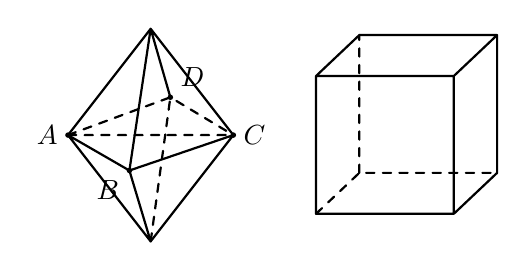
\begin{tikzpicture}[line cap=round,line join=round,thick]
  % Two congruent square pyramids sharing the square ABCD.
  \coordinate (A) at (0,1.0); \coordinate (B) at (0.78,0.55);
  \coordinate (C) at (2.1,1.0); \coordinate (D) at (1.30,1.48);
  \coordinate (T) at (1.05,2.35); \coordinate (S) at (1.05,-0.35);
  \draw[dashed] (A)--(C) (A)--(D)--(C) (S)--(D);
  \draw (A)--(B)--(C) (T)--(A) (T)--(B) (T)--(D) (T)--(C)
        (S)--(A) (S)--(B) (S)--(C);
  \fill (A) circle (1pt) node[left] {$A$};
  \fill (B) circle (1pt) node[below left] {$B$};
  \fill (C) circle (1pt) node[right] {$C$};
  \fill (D) circle (1pt) node[above right] {$D$};
  % Unit cube; hidden rear-left edges are dashed.
  \begin{scope}[xshift=3.15cm]
    \coordinate (a) at (0,0); \coordinate (b) at (1.75,0);
    \coordinate (c) at (1.75,1.75); \coordinate (d) at (0,1.75);
    \coordinate (e) at (0.55,0.52); \coordinate (f) at (2.3,0.52);
    \coordinate (g) at (2.3,2.27); \coordinate (h) at (0.55,2.27);
    \draw (a)--(b)--(c)--(d)--cycle (b)--(f)--(g)--(c) (d)--(h)--(g);
    \draw[dashed] (a)--(e)--(f) (e)--(h);
  \end{scope}
\end{tikzpicture}
\end{center}
\nopagebreak[4]
\Needspace{4\baselineskip}
\textbf{解析}

\Needspace{5\baselineskip}
取单位正方体 $[0,1]^3$，令共同底面位于 $z=1/2$，中心为 $(1/2,1/2,1/2)$。设底面正方形外接圆半径为 $R$，其顶点方向与坐标轴夹角为 $\theta\in[0,\pi/4]$，并令 $R\cos\theta=1/2$。四个顶点的坐标偏移为 $(\pm R\cos\theta,\pm R\sin\theta)$ 的轮换，因此每个顶点均落在正方体某个侧面上；上下两个锥顶分别取 $(1/2,1/2,0)$ 与 $(1/2,1/2,1)$，也在正方体表面。两锥高各为 $1/2$，底面积为 $2R^2=1/(2\cos^2\theta)$，整体体积
\nopagebreak[4]
\[V=2\cdot\frac13\cdot\frac12\cdot2R^2=\frac1{6\cos^2\theta}.\]
当 $\theta$ 连续取 $[0,\pi/4]$ 时，$V$ 连续取 $[1/6,1/3]$ 中所有值，可能体积有无穷多个，故选 D。此构造证明“可能值无穷多”即可，无须穷尽其他嵌入。

\gkanswer{答案：D（无穷多个）。}

\end{answer}
\begin{answer}
\gksolhead{10}{}

\textbf{题目}：

图中有一个信号源和五个接收器。接收器与信号源在同一个串联线路中时，就能接收到信号，否则就不能接收到信号。若将图中左端的六个接线点随机地平均分成三组，将右端的六个接线点也随机地平均分成三组，再把所有六组中每组的两个接线点用导线连接，则这五个接收器能同时接收到信号的概率是\mbox{（　　）}

\begin{gkopts}(2)
\task （A）$\dfrac{4}{45}$
\task （B）$\dfrac{1}{36}$
\task （C）$\dfrac{4}{15}$
\task （D）$\dfrac{8}{15}$
\end{gkopts}
\nopagebreak[4]
\begin{center}% Source-relative PDF page 1, Q10 (printed page 302).
\begin{tikzpicture}[line cap=round,line join=round,thick]
  \foreach \y in {0,-0.62,-1.24,-1.86,-2.48,-3.10} {
    \draw (0,\y)--(4.4,\y);
    \fill (0,\y) circle (1.15pt);
    \fill (4.4,\y) circle (1.15pt);
  }
  \draw (2.2,0) circle (0.24);
  \draw (2.2,0) circle (0.085);
  \node[above=5pt] at (2.2,0.24) {信号源};
  \foreach \y in {-0.62,-1.24,-1.86,-2.48,-3.10}
    \draw (1.82,\y-0.15) rectangle (2.58,\y+0.15);
\end{tikzpicture}
\end{center}
\nopagebreak[4]
\Needspace{4\baselineskip}
\textbf{解析}

每侧的六个接线点随机配成三对，等价于在六个支路标签上取一个完美匹配；共有 $(6-1)!!=15$ 种，左右独立。固定左侧匹配后，右侧也有 15 种。要使信号源和五个接收器都在同一个串联回路，两个匹配的并图必须是一个含六个顶点的交替六环。把左侧三对收缩为三个点，右侧配对必须在这三对之间连成三角形；对每个左侧配对，两个端点可分别接向相邻两对，故有 $2^3=8$ 种右侧匹配，且这些匹配互异。因此概率为 $8/15$，选 D。

\gkanswer{答案：D（$\dfrac8{15}$）。}

\end{answer}
\begin{answer}
\gksolhead{11}{}

\textbf{题目}：

在 $\triangle ABC$ 中，已知 $BC=12$，$A=60^\circ$，$B=45^\circ$，则 $AC=$ \gkblank{}。

\Needspace{4\baselineskip}
\textbf{解析}

正弦定理给出 $AC/\sin45^\circ=BC/\sin60^\circ$，所以 $AC=12\cdot(\sqrt2/2)/(\sqrt3/2)=4\sqrt6$。

\gkanswer{答案：$4\sqrt6$。}

\end{answer}
\begin{answer}
\gksolhead{12}{}

\textbf{题目}：

\Needspace{5\baselineskip}
设变量 $x,y$ 满足约束条件
\nopagebreak[4]
\[\begin{cases}2x-y\leqslant2,\\x-y\geqslant-1,\\x+y\geqslant1,\end{cases}\]
则 $z=2x+3y$ 的最大值为 \gkblank{}。

\Needspace{4\baselineskip}
\textbf{解析}

可行域顶点由三条边界线两两相交得到 $(0,1),(1,0),(3,4)$。目标函数 $2x+3y$ 在三点处分别为 $3,2,18$，最大值为 $18$。

\gkanswer{答案：18。}

\end{answer}
\begin{answer}
\gksolhead{13}{}

\textbf{题目}：

今有 2 个红球，3 个黄球，4 个白球，同色球不加以区分，将这 9 个球排成一列有 \gkblank{} 种不同的方法。（用数字作答）

\Needspace{4\baselineskip}
\textbf{解析}

相同颜色球不可区分，排列数为 $9!/(2!3!4!)=1260$。

\gkanswer{答案：1260。}

\end{answer}
\begin{answer}
\gksolhead{14}{}

\textbf{题目}：

$\cot20^\circ\cos10^\circ+\sqrt3\sin10^\circ\tan70^\circ-2\cos40^\circ=$ \gkblank{}。

\Needspace{4\baselineskip}
\textbf{解析}

利用 $\tan70^\circ=\cot20^\circ$ 及 $\cos10^\circ+\sqrt3\sin10^\circ=2\cos50^\circ=2\sin40^\circ$，原式化为 $2\sin40^\circ\cos20^\circ/\sin20^\circ-2\cos40^\circ=4\cos^2 20^\circ-2\cos40^\circ=2$。

\gkanswer{答案：2。}

\end{answer}
\begin{answer}
\gksolhead{15}{}

\textbf{题目}：

对正整数 $n$，设曲线 $y=x^n(1-x)$ 在 $x=2$ 处的切线与 $y$ 轴交点的纵坐标为 $a_n$，则数列 $\left\{\dfrac{a_n}{n+1}\right\}$ 的前 $n$ 项和的公式是 \gkblank{}。

\Needspace{4\baselineskip}
\textbf{解析}

令 $F(x)=x^n(1-x)$。则 $F(2)=-2^n$、$F'(2)=-(n+2)2^{n-1}$。切线纵截距 $a_n=F(2)-2F'(2)=(n+1)2^n$，故 $a_n/(n+1)=2^n$，前 $n$ 项和为 $2^{n+1}-2$。

\gkanswer{答案：$2^{n+1}-2$。}

\end{answer}
\begin{answer}
\gksolhead{16}{}

\textbf{题目}：

不等式 $\log_2\left(x+\dfrac1x+6\right)\leqslant3$ 的解集为 \gkblank{}。

\Needspace{4\baselineskip}
\textbf{解析}

还须满足对数真数为正。令 $u=x+1/x$，原式等价于 $-6<u\le2$ 且 $x\ne0$。当 $x>0$ 时 $u\ge2$，并且等号仅在 $x=1$，故正数解只有 $x=1$。当 $x<0$ 时 $u\le-2$，上界自动满足；下界 $x+1/x>-6$ 两边乘以负数 $x$ 并移项，等价于 $x^2+6x+1<0$。其根为 $-3\pm2\sqrt2$，故负数解为 $(-3-2\sqrt2,-3+2\sqrt2)$。合并得 $(-3-2\sqrt2,-3+2\sqrt2)\cup\{1\}$。

\gkanswer{答案：$(-3-2\sqrt2,-3+2\sqrt2)\cup\{1\}$。}

\end{answer}
\begin{answer}
\gksolhead{17}{}

\textbf{题目}：

已知三点 $P(5,2)\text{、}F_1(-6,0)\text{、}F_2(6,0)$。

（1） 求以 $F_1\text{、}F_2$ 为焦点且过点 $P$ 的椭圆的标准方程；

（2） 设点 $P\text{、}F_1\text{、}F_2$ 关于直线 $y=x$ 的对称点分别为 $P'\text{、}F_1'\text{、}F_2'$，求以 $F_1'\text{、}F_2'$ 为焦点且过点 $P'$ 的双曲线的标准方程。

\Needspace{4\baselineskip}
\textbf{解析}

\gksubpart{(1)}

焦点距 $c=6$。$PF_1=5\sqrt5$、$PF_2=\sqrt5$，故 $2a=6\sqrt5$，$a=3\sqrt5$，$b^2=a^2-c^2=9$。标准方程为 $x^2/45+y^2/9=1$。

\gksubpart{(2)}

关于 $y=x$ 对称后，焦点为 $(0,-6),(0,6)$，点为 $(2,5)$。其到两焦点距离为 $5\sqrt5$ 与 $\sqrt5$，差为 $4\sqrt5=2a$，故 $a=2\sqrt5$、$c=6$、$b^2=16$。双曲线方程为 $y^2/20-x^2/16=1$。

\gkanswer{答案（1）：$\frac{x^2}{45}+\frac{y^2}{9}=1$。}

\gkanswer{答案（2）：$\frac{y^2}{20}-\frac{x^2}{16}=1$。}

\end{answer}
\begin{answer}
\gksolhead{18}{}

\textbf{题目}：

请您设计一个帐篷。它下部的形状是高为 $1\text{ m}$ 的正六棱柱，上部的形状是侧棱长为 $3\text{ m}$ 的正六棱锥（如图所示）。试问当帐篷的顶点 $O$ 到底面中心 $O_1$ 的距离为多少时，帐篷的体积最大？
\nopagebreak[4]
\begin{center}% Source-relative PDF page 1, Q18 (printed page 302).
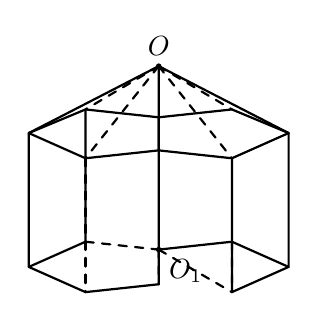
\begin{tikzpicture}[line cap=round,line join=round,thick]
  % Upper hexagonal pyramid, joined to a hexagonal prism below.
  \coordinate (O) at (1.65,3.65);
  \coordinate (A) at (0,2.8); \coordinate (B) at (0.72,3.1);
  \coordinate (C) at (1.65,3.0); \coordinate (D) at (2.58,3.1);
  \coordinate (E) at (3.3,2.8); \coordinate (F) at (2.58,2.48);
  \coordinate (G) at (1.65,2.58); \coordinate (H) at (0.72,2.48);
  \coordinate (I) at (0,1.1); \coordinate (J) at (0.72,1.42);
  \coordinate (K) at (1.65,1.32); \coordinate (L) at (2.58,1.42);
  \coordinate (M) at (3.3,1.1); \coordinate (N) at (2.58,0.78);
  \coordinate (Q) at (1.65,0.88); \coordinate (R) at (0.72,0.78);
  \draw (A)--(B)--(C)--(D)--(E) (E)--(F)--(G)--(H)--(A);
  \draw (O)--(A) (O)--(C) (O)--(E) (O)--(G);
  \draw[dashed] (O)--(B) (O)--(D) (O)--(F) (O)--(H);
  \draw (A)--(I)--(J)--(B) (C)--(K)--(G) (E)--(M)--(N)--(F);
  \draw (I)--(R)--(Q)--(K)--(L)--(M);
  \draw[dashed] (J)--(K) (J)--(R) (K)--(Q) (K)--(N) (L)--(N);
  \draw[dashed] (H)--(R) (G)--(Q) (F)--(N);
  \fill (O) circle (1pt) node[above] {$O$};
  \fill (K) circle (1pt) node[below right] {$O_1$};
\end{tikzpicture}
\end{center}
\nopagebreak[4]
\Needspace{4\baselineskip}
\textbf{解析}

\Needspace{5\baselineskip}
令正六边形底面外接圆半径为 $r$，帐篷顶点到底面中心的高度为 $h$。正六棱锥侧棱长为 3，故 $r^2+h^2=9$。底面积为 $3\sqrt3r^2/2$，总体积为
\nopagebreak[4]
\[
V=\frac{3\sqrt3}{2}(9-h^2)(1+h/3),\qquad 0\le h\le3.
\]
去掉正因子后，对 $(9-h^2)(1+h/3)$ 求导，驻点满足 $h^2+2h-3=0$。区间 $[0,3]$ 内解为 $h=1$；端点 $h=0,3$ 均给出更小体积，故最大值在 $h=1$ 处取得。

\gkanswer{答案：$OO_1=1$ m。}

\end{answer}
\begin{answer}
\gksolhead{19}{}

\textbf{题目}：

在正三角形 $ABC$ 中，$E\text{、}F\text{、}P$ 分别是 $AB\text{、}AC\text{、}BC$ 边上的点，满足 $AE:EB=CF:FA=CP:PB=1:2$（如图 1）。将 $\triangle AEF$ 沿 $EF$ 折起到 $\triangle A_1EF$ 的位置，使二面角 $A_1-EF-B$ 成直二面角，连接 $A_1B\text{、}A_1P$（如图 2）。

（1） 求证：$A_1E\perp$ 平面 $BEP$；

（2） 求直线 $A_1E$ 与平面 $A_1BP$ 所成角的大小；

（3） 求二面角 $B-A_1P-F$ 的大小。（用反三角函数表示）
\nopagebreak[4]
\begin{center}% Source-relative PDF page 2, Q19 (printed page 303); left=图1, right=图2.
\begin{tikzpicture}[line cap=round,line join=round,thick]
  % 图1: equilateral triangle ABC, with E,F,P on the indicated sides.
  \begin{scope}
    \coordinate (A) at (1.25,2.45); \coordinate (B) at (0,0); \coordinate (C) at (2.5,0);
    \coordinate (E) at (0.42,0.82); \coordinate (F) at (2.08,0.82);
    \coordinate (P) at (1.67,0);
    \draw (A)--(B)--(C)--cycle (E)--(F) (P)--(F);
    \foreach \p/\pos in {A/above,B/below left,C/below right,E/left,F/above right,P/below}
      \fill (\p) circle (0.9pt) node[\pos] {$\p$};
    \node[below=5pt] at (1.25,-0.3) {图 1};
  \end{scope}
  \node at (3.15,1.15) {$\Longrightarrow$};
  % 图2: folded solid; hidden edges and the EF hinge continuation are dashed.
  \begin{scope}[xshift=3.8cm]
    \coordinate (B) at (0,0); \coordinate (P) at (1.5,0); \coordinate (C) at (2.6,0);
    \coordinate (Aone) at (1.48,1.65); \coordinate (E) at (1.42,0.70);
    \coordinate (F) at (2.23,0.54);
    \draw (B)--(P)--(C) (B)--(Aone)--(C) (Aone)--(P) (P)--(F)--(C);
    \draw[dashed] (Aone)--(E) (B)--(E)--(F) (E)--(P);
    \foreach \p/\pos in {B/below left,C/below right,E/left,F/right,P/below}
      \fill (\p) circle (0.9pt) node[\pos] {$\p$};
    \fill (Aone) circle (0.9pt) node[above] {$A_1$};
    \node[below=5pt] at (1.3,-0.3) {图 2};
  \end{scope}
\end{tikzpicture}
\end{center}
\nopagebreak[4]
\Needspace{4\baselineskip}
\textbf{解析}

\gksubpart{(1) 证明 $A_1E$ 垂直平面 $BEP$}

取边长为 3 的坐标系 $B=(0,0,0),C=(3,0,0),A=(\frac32,\frac{3\sqrt3}2,0)$。由比例关系得 $E=(1,\sqrt3,0),F=(\frac52,\frac{\sqrt3}2,0),P=(2,0,0)$。先有 $\overrightarrow{EA}=(\frac12,\frac{\sqrt3}2,0)$、$\overrightarrow{EF}=(\frac32,-\frac{\sqrt3}2,0)$，故 $EA\perp EF$。折起使平面 $A_1EF$ 与平面 $BEF$ 垂直，因此 $A_1E\perp BE$ 且 $A_1E\perp EF$；又 $BE,EF$ 是平面 $BEP$ 内相交直线，故 $A_1E\perp\text{\text{平面} }BEP$。

\gksubpart{(2) 线面角}

取折起方向为正 $z$ 方向，则 $A_1=(1,\sqrt3,1)$，直线 $A_1E$ 的方向向量可取 $\mathbf u=(0,0,1)$。平面 $A_1BP$ 的法向量可取 $\mathbf n=(0,-1,\sqrt3)$，$|\mathbf n|=2$。线面角 $\alpha$ 满足 $\sin\alpha=|\mathbf u\cdot\mathbf n|/(|\mathbf u||\mathbf n|)=\sqrt3/2$，故 $\alpha=60^\circ$。

\gksubpart{(3) 二面角}

\Needspace{5\baselineskip}
令棱 $A_1P$ 的方向向量 $\mathbf u=(1,-\sqrt3,-1)$，另取 $\mathbf v=\overrightarrow{A_1B}=(-1,-\sqrt3,-1)$、$\mathbf w=\overrightarrow{A_1F}=(\frac32,-\frac{\sqrt3}2,-1)$。将 $\mathbf v,\mathbf w$ 投影到垂直于棱 $A_1P$ 的平面，投影点积为
\nopagebreak[4]
\[\mathbf v\cdot\mathbf w-\frac{(\mathbf v\cdot\mathbf u)(\mathbf w\cdot\mathbf u)}{\mathbf u\cdot\mathbf u}=1-\frac{3\cdot4}{5}=-\frac75.\]
两投影向量长度分别为 $4/\sqrt5$、$2/\sqrt5$，故其夹角余弦为 $(-7/5)/(8/5)=-7/8$。按二面角 $B-A_1P-F$ 的两面内射线方向取角，所得为钝角 $\arccos(-7/8)$。

\gkanswer{答案（1）：见解析版}

\gkanswer{答案（2）：$60^\circ$。}

\gkanswer{答案（3）：$\arccos(-\frac78)$。}

\end{answer}
\begin{answer}
\gksolhead{20}{}

\textbf{题目}：

设 $a$ 为实数，设函数 $f(x)=a\sqrt{1-x^2}+\sqrt{1+x}+\sqrt{1-x}$ 的最大值为 $g(a)$。

（1） 设 $t=\sqrt{1+x}+\sqrt{1-x}$，求 $t$ 的取值范围，并把 $f(x)$ 表示为 $t$ 的函数 $m(t)$；

（2） 求 $g(a)$；

（3） 试求满足 $g(a)=g\left(\dfrac1a\right)$ 的所有实数 $a$。

\Needspace{4\baselineskip}
\textbf{解析}

\gksubpart{(1)}

由 $t^2=2+2\sqrt{1-x^2}$ 得 $t\in[\sqrt2,2]$，且 $\sqrt{1-x^2}=(t^2-2)/2$。因此 $m(t)=\frac a2(t^2-2)+t$。

\gksubpart{(2)}

对 $m$ 关于 $t$ 求导，$m'(t)=at+1$。当 $a\le-1/\sqrt2$ 时，函数在区间上不增，最大值 $m(\sqrt2)=\sqrt2$。当 $-1/\sqrt2<a<-1/2$ 时，驻点 $t=-1/a$ 在区间内部，最大值为 $m(-1/a)=-1/(2a)-a$。当 $a\ge-1/2$ 时，最大值取在 $t=2$，为 $a+2$。边界处相邻表达式一致。

\gksubpart{(3)}

令 $a\ne0$，按 $a$ 与 $1/a$ 所属分段分类。若 $a>0$，两者均属于 $a\ge-1/2$ 段，等式化为 $a+2=1/a+2$，故 $a=1$。若 $a<0$ 且 $a\in[-\sqrt2,-1/\sqrt2]$，则 $a$ 与 $1/a$ 都落在 $a\le-1/\sqrt2$ 段，二者函数值均为 $\sqrt2$。若 $a\le-2$，则 $g(a)=\sqrt2$、$g(1/a)=1/a+2$，解得 $a=-(2+\sqrt2)$，且满足本段条件。其余负数区间按相邻段公式相等求解，所得边界解仅为已列出的 $a=-\sqrt2$、$a=-1/\sqrt2$，内部方程无新解。因此全部解为 $\{1\}\cup[-\sqrt2,-1/\sqrt2]\cup\{-2-\sqrt2\}$；$a=0$ 不在定义域内。

\gkanswer{答案（1）：$t\in[\sqrt2,2]$，$m(t)=\frac a2(t^2-2)+t$。}

\gkanswer{答案（2）：若 $a\le-1/\sqrt2$，$g(a)=\sqrt2$；若 $-1/\sqrt2<a<-1/2$，$g(a)=-\frac1{2a}-a$；若 $a\ge-1/2$，$g(a)=a+2$。}

\gkanswer{答案（3）：$a\in\{1\}\cup[-\sqrt2,-1/\sqrt2]\cup\{-2-\sqrt2\}$。}

\end{answer}
\begin{answer}
\gksolhead{21}{}

\textbf{题目}：

设数列 $\{a_n\},\{b_n\},\{c_n\}$ 满足：$b_n=a_n-a_{n+2}$，$c_n=a_n+2a_{n+1}+3a_{n+2}$（$n=1,2,3,\cdots$）。证明：$\{a_n\}$ 为等差数列的充分必要条件是 $\{c_n\}$ 为等差数列且 $b_n\leqslant b_{n+1}$（$n=1,2,3,\cdots$）。

\Needspace{4\baselineskip}
\textbf{解析}

\gksubpart{充分性}

设 $a_n$ 为等差数列，公差为 $d$。则 $b_n=a_n-a_{n+2}=-2d$ 为常数列，满足 $b_n\le b_{n+1}$；而 $c_n=a_n+2a_{n+1}+3a_{n+2}$ 是关于 $n$ 的一次数列，故为等差数列。

\gksubpart{必要性}

\Needspace{5\baselineskip}
设 $d_n=a_{n+1}-a_n$。由 $b_n=-(d_n+d_{n+1})$ 及 $b_n\le b_{n+1}$，得 $d_n\ge d_{n+2}$，故偶数项列与奇数项列分别单调不增。又 $c_n$ 为等差数列，所以 $q_n=c_{n+1}-c_n=d_n+2d_{n+1}+3d_{n+2}$ 为常数。令 $x_k=d_{2k}$、$y_k=d_{2k+1}$；两列均单调不增，且
\nopagebreak[4]
\[
q_{2k}=x_k+2y_k+3x_{k+1}=q_{2k+2}=x_{k+1}+2y_{k+1}+3x_{k+2}.
\]
\Needspace{5\baselineskip}
因此
\nopagebreak[4]
\[
(x_k-x_{k+1})+2(y_k-y_{k+1})+3(x_{k+1}-x_{k+2})=0.
\]
三项均非负，故各项为零，得到 $x_k=x_{k+1}=x_{k+2}$、$y_k=y_{k+1}$；对所有 $k$ 成立，说明奇数位差分为常数 $y$、偶数位差分为常数 $x$。再由 $q_{2k}=q_{2k+1}$ 得 $x+2y+3x=y+2x+3y$，从而 $x=y$。故所有 $d_n$ 相等，$\{a_n\}$ 为等差数列。

\gkanswer{答案：充分必要性成立（证明见解析）。}

\end{answer}